\section{Height of sensors} \label{sec:height}
A definition on how to place the different sensors on the turtlebot is needed to get the desired readings for this project.

\subsection{Height of LIDAR}
%why not torso
When emitting the laser pulse it is scanning in a 270\degree \space horizontal FOV. So it is needed to target the LIDAR to a specific height to eliminate the unwanted body parts.\\
There is two known scanning methods for body parts, that is familiar with this project, when detecting people with a LIDAR: torso scanning and leg detection.
Torso scanning is a widely used detection tool. The scanning takes use of clusters, which is a high-level description of the image content. This is the same as having a lot of features matching the described picture so that the classifier is integrated on a desirable level. However, it is seen that torso scanning readings does not provide much information for the detection and classification of the objects, but can be used for tracking purposes \cite{taipalus2011human}. 
Another approach is to scan for the legs. This is based on the geometric features to estimate the centre of the person it is scanning by the persons leg placement, which is why 0.56 meters (knee-height) LIDAR scanning is reasonable  \cite{taipalus2011human}.

\subsection{Height of depth camera}
As the camera is used for face detection, it must be placed at a height for which it can capture faces from a wide range of height of people. We assume that the people using the robotic solution will be less than 2m tall and the robot should be compliant with personal space, which is about 1.2m, as mentioned in requirement 1.3.
To be able to capture images of anyone below 2m tall at a distance of 1.2m the Intel Real Sense camera must be placed in a height of 1.35m. This is due to the field of view of the camera being 57\degree vertically. The distance calculation can be seen in figure \ref{fig:RealSenseAngle}. As the field of view also goes downwards the lowest height of a person at the distance of 1.2m from the camera is 0.7m. This enables the detection of most people in a hypermarket.

\begin{figure}[H]
    \centering
    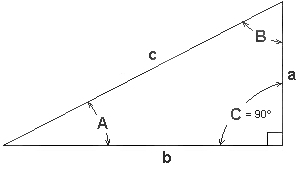
\includegraphics[width=.75\textwidth]{figures/Triangle.png}
    \caption{Triangle for calculating the height of people found in the FOV at 1.2m distance. A = 28.5\degree, b=1.2m, a=0.65m. The camera is placed at the angle A and the person on the side a with b being the distance of 1.2 between the camera and the person.}
    \label{fig:RealSenseAngle}
\end{figure}

With the needed sensors described the description of the physical setup of the prototype robot can be completed.